\documentclass{article}

\usepackage[portuguese]{babel}

\usepackage{amsmath, amssymb}
\usepackage{graphicx}
\usepackage{listings}
\usepackage[shortlabels]{enumitem}
\usepackage[colorlinks=true, allcolors=blue]{hyperref}

\usepackage[section]{placeins}

\title{Relatório 04}
\author{Vinícius de Oliveira Peixoto Rodrigues (245294)}
\date{Setembro de 2022}

\begin{document}
\maketitle

\section*{Questão 1}

Como o site do DCA redireciona para a versão HTTPS independentemente do request, foi usado aqui o site \url{www.neverssl.com}.

\subsection*{Item (a)}

Request \texttt{HEAD}:

\begin{verbatim}
    HTTP/1.1 200 OK
    Date: Wed, 21 Sep 2022 12:50:27 GMT
    Server: Apache/2.4.53 ()
    Upgrade: h2,h2c
    Connection: Upgrade
    Last-Modified: Wed, 29 Jun 2022 00:23:33 GMT
    ETag: "f79-5e28b29d38e93"
    Accept-Ranges: bytes
    Content-Length: 3961
    Vary: Accept-Encoding
    Content-Type: text/html; charset=UTF-8
\end{verbatim}

Percebe-se que para o \texttt{OPTIONS} foi recebido o campo \texttt{Allow}, indicando os requests HTTP aceitos; foram também omitidos vários campos presentes no \texttt{HEAD}.

\subsection*{Item (b)}

\begin{verbatim}
    HTTP/1.1 200 OK
    Date: Wed, 21 Sep 2022 12:54:27 GMT
    Server: Apache/2.4.53 ()
    Transfer-Encoding: chunked
    Content-Type: message/http

    2c
    TRACE / HTTP/1.1
    Host: www.neverssl.com


    0

\end{verbatim}

Percebe-se que, como esperado, o servidor recebeu o request (\texttt{200 OK}) e enviou de volta a mensagem que recebeu (\texttt{TRACE / HTTP/1.1...}).

\subsection*{Item (c)}

\begin{verbatim}
    HTTP/1.1 200 OK
    Date: Wed, 21 Sep 2022 12:57:13 GMT
    Server: Apache/2.4.53 ()
    Upgrade: h2,h2c
    Connection: Upgrade
    Last-Modified: Wed, 29 Jun 2022 00:23:33 GMT
    ETag: "f79-5e28b29d38e93"
    Accept-Ranges: bytes
    Content-Length: 3961
    Vary: Accept-Encoding
    Content-Type: text/html; charset=UTF-8

    <html>
        <!╌ CÓDIGO-FONTE DA PÁGINA INICIAL ╌>
    </html>
\end{verbatim}

Como o request de \texttt{POST} foi enviado vazio, o servidor retornou de volta a página inicial (o recurso pro qual mandamos o \texttt{POST}, localizado em \texttt{/}).

\subsection*{Item (d)}

\begin{verbatim}
    HTTP/1.1 405 Method Not Allowed
    Date: Wed, 21 Sep 2022 13:03:25 GMT
    Server: Apache/2.4.53 ()
    Allow: OPTIONS,HEAD,GET,POST,TRACE
    Content-Length: 223
    Content-Type: text/html; charset=iso-8859-1
    
    <!DOCTYPE HTML PUBLIC "-//IETF//DTD HTML 2.0//EN">
    <html><head>
    <title>405 Method Not Allowed</title>
    </head><body>
    <h1>Method Not Allowed</h1>
    <p>The requested method DELETE is not allowed for this URL.</p>
    </body></html>     
\end{verbatim}

O servidor retornou \texttt{405 Method Not Allowed}, como era de se esperar (visto que o request \texttt{DELETE} não estava listado como disponível no \texttt{OPTIONS} do item (a)).

\subsection*{Item (e)}

\begin{verbatim}
    HTTP/1.1 501 Not Implemented
    Date: Wed, 21 Sep 2022 13:05:01 GMT
    Server: Apache/2.4.53 ()
    Allow: OPTIONS,HEAD,GET,POST,TRACE
    Content-Length: 208
    Connection: close
    Content-Type: text/html; charset=iso-8859-1

    <!DOCTYPE HTML PUBLIC "-//IETF//DTD HTML 2.0//EN">
    <html><head>
    <title>501 Not Implemented</title>
    </head><body>
    <h1>Not Implemented</h1>
    <p>AGORA_VAI not supported for current URL.<br />
    </p>
    </body></html>
\end{verbatim}

O servidor retornou um \texttt{501 Not Implemented}, também conforme o esperado, visto que o \texttt{AGORA\_VAI} não é um request válido do HTTP.

\section*{Questão 2}
A linha \texttt{Host} serve para se referir a hosts \textit{virtuais} (i.e., configurados na máquina host para a qual mandamos o request). Caso o servidor não possua hosts virtuais, a linha não faz efeito:

\begin{verbatim}
    > telnet www.neverssl.com 80
    Trying 34.223.124.45...
    Connected to www.neverssl.com.
    Escape character is '^]'.
    GET / HTTP/1.1
    Host: www.example.com

    HTTP/1.1 200 OK
    Date: Wed, 21 Sep 2022 13:14:32 GMT
    Server: Apache/2.4.53 ()
    Upgrade: h2,h2c
    Connection: Upgrade
    Last-Modified: Wed, 29 Jun 2022 00:23:33 GMT
    ETag: "f79-5e28b29d38e93"
    Accept-Ranges: bytes
    Content-Length: 3961
    Vary: Accept-Encoding
    Content-Type: text/html; charset=UTF-8

    <html>
        <!╌ CÓDIGO-FONTE DA PÁGINA INICIAL ╌>
    </html>
\end{verbatim}

\begin{verbatim}
    > telnet www.dca.fee.unicamp.br 80
    Trying 143.106.148.94...
    Connected to www.dca.fee.unicamp.br.
    Escape character is '^]'.
    GET / HTTP/1.1
    Host: www.unicamp.br

    HTTP/1.1 302 Found
    Date: Wed, 21 Sep 2022 13:17:49 GMT
    Server: Apache
    Location: https://www.dca.fee.unicamp.br/
    Content-Length: 215
    Content-Type: text/html; charset=iso-8859-1

    <!DOCTYPE HTML PUBLIC "-//IETF//DTD HTML 2.0//EN">
    <html><head>
    <title>302 Found</title>
    </head><body>
    <h1>Found</h1>
    <p>The document has moved <a href="https://www.dca.fee.unicamp.br/">here</a>.</p>
    </body></html>
\end{verbatim}

\section*{Questão 3}

\begin{enumerate}[(a)]
    \item \texttt{200 OK}: indica que não houveram erros com o request
    \item \texttt{400 Bad Request}: indica que houve algum erro (da parte do cliente) com o request, de modo que o servidor se recusa a responder
    \item \texttt{401 Unauthorized}: indica que as credenciais do cliente são inválidas
    \item \texttt{403 Forbidden}: indica que o cliente não tem privilégio suficiente para fazer um request
    \item \texttt{404 Not Found}: indica que um recurso não foi encontrado no servidor
    \item \texttt{405 Method Not Allowed}: indica que o servidor não aceita requests com o método utilizado
    \item \texttt{500 Internal Server Error}: indica que houve um erro interno da parte do servidor que impossibilitou o processamento do request
    \item \texttt{501 Not Implemented}: indica que o servidor não reconheceu um método (seja porque é inválido ou porque o servidor não tem suporte para ele)
    \item \texttt{Accept-Ranges}: especifica se o servidor suporta enviar um range específico de bytes do resource solicitado (útil para fazer download de um arquivo em chunks, por exemplo)
    \item \texttt{Allow}: lista os métodos suportados por um recurso
    \item \texttt{ETag} (Entity Tag): indica a versão específica de um recurso
    \item \texttt{X-Pad}: um header que faz um padding da resposta do servidor como uma forma de contornar um bug relacionado ao tamanho do response header em alguns browsers antigos
    \item \texttt{Content-Length}: o tamanho da mensagem de resposta, em bytes
    \item \texttt{Content-Type}: indica o tipo do recurso (normalmente usado para mídia)
    \item \texttt{Date}: indica a data em que a mensagem de resposta foi criada
    \item \texttt{Last-Modified}: indica a última data em que um recurso foi modificado (útil para determinar se é necessário fazer refetch de um recurso ou se é possível usar a versão armazenada em cache)
    \item \texttt{Server}: indica o software utilizado pelo servidor que gerou a resposta
    \item \texttt{Transfer-Encoding}: especifica o encoding utilizado no corpo da resposta
    \item \texttt{WWW-Authenticate}: define os métodos de autenticação utilizados para ganhar acesso a um recurso
    \item \texttt{Chunked}: modo de transferência em stream onde um recurso grande é enviado em chunks (blocos pequenos) em vez de por completo
\end{enumerate}

\section*{Questão 4}

\begin{verbatim}
    > telnet www.example.com 80
    DELETE / HTTP/1.1
    Host: www.example.com

    HTTP/1.1 405 Method Not Allowed
    Cache-Control: max-age=604800
    Content-Type: text/html; charset=UTF-8
    Date: Wed, 21 Sep 2022 13:47:24 GMT
    Expires: Wed, 28 Sep 2022 13:47:24 GMT
    Server: EOS (vny/0453)
    Content-Length: 0

    GET /aljksdajsd HTTP/1.1
    Host: www.example.com

    HTTP/1.1 404 Not Found
    Cache-Control: max-age=604800
    Content-Type: text/html; charset=UTF-8
    Date: Wed, 21 Sep 2022 13:48:33 GMT
    Expires: Wed, 28 Sep 2022 13:48:33 GMT
    Server: EOS (vny/044E)
    Vary: Accept-Encoding
    Content-Length: 1256

    klasjdasd

    HTTP/1.0 501 Not Implemented
    Content-Type: text/html
    Content-Length: 357
    Connection: close
    Date: Wed, 21 Sep 2022 13:49:34 GMT
    Server: ECSF (mic/9AE2)

    GET / HTTP/1.1

    HTTP/1.1 400 Bad Request
    Content-Type: text/html
    Content-Length: 349
    Connection: close
    Date: Wed, 21 Sep 2022 13:50:12 GMT
    Server: ECSF (mic/9B4F)

    GET / HTTP/123.2

    HTTP/1.0 505 HTTP Version Not Supported
    Content-Type: text/html
    Content-Length: 379
    Connection: close
    Date: Wed, 21 Sep 2022 14:01:21 GMT
    Server: ECSF (mic/9AF8)
\end{verbatim}

\section*{Questão 5}

O servidor retorna o seguinte:

\begin{verbatim}
    GET / HTTP/1.1
    Host: www.dca.fee.unicamp.br

    HTTP/1.1 302 Found
    Date: Wed, 21 Sep 2022 14:11:47 GMT
    Server: Apache
    Location: https://www.dca.fee.unicamp.br/
    Content-Length: 215
    Content-Type: text/html; charset=iso-8859-1

    <!DOCTYPE HTML PUBLIC "-//IETF//DTD HTML 2.0//EN">
    <html><head>
    <title>302 Found</title>
    </head><body>
    <h1>Found</h1>
    <p>The document has moved <a href="https://www.dca.fee.unicamp.br/">here</a>.</p>
    </body></html>
\end{verbatim}

De modo a indicar para o navegador que o recurso foi movido para um outro endereço que só aceita o protocolo HTTPS.

\newpage
\section*{Item (b)}

Como não é possível se comunicar via telnet com o servidor para fazer os vários \texttt{GET} que montam a página completa, estou deixando documentado aqui os vários requests de recursos diferentes na página que o navegador faz para montar a versão final:

\begin{figure}[!ht]
    \begin{center}
        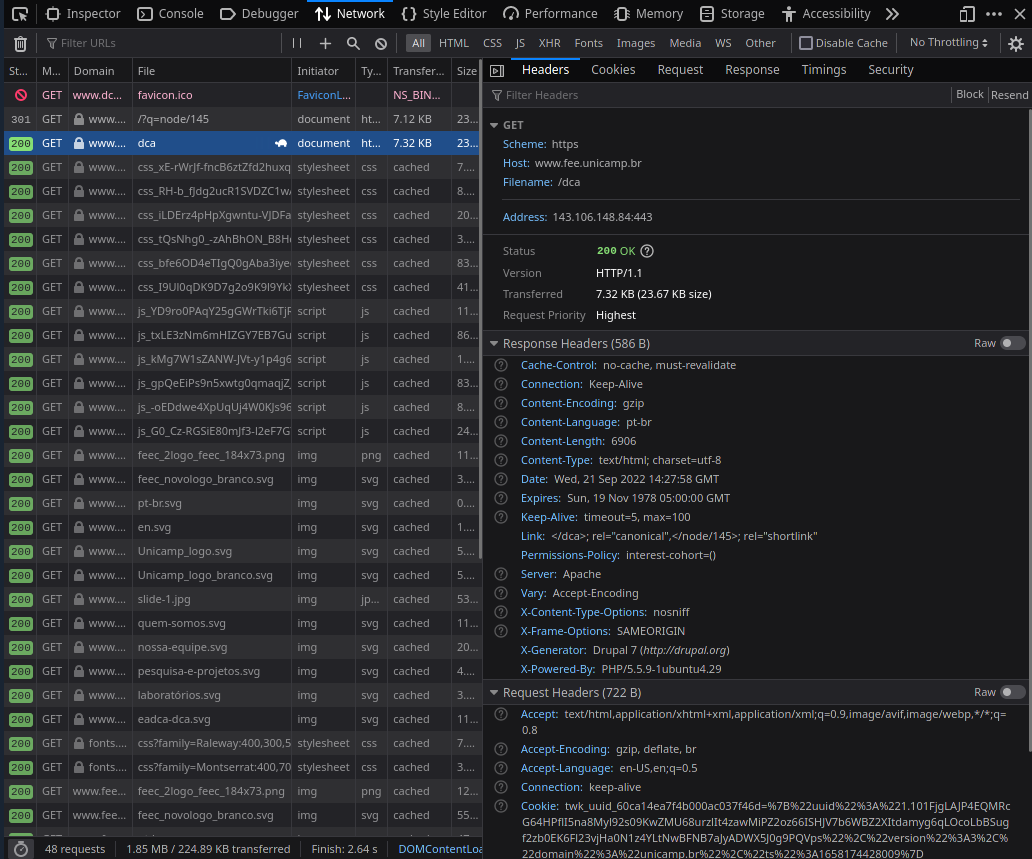
\includegraphics[width=\textwidth]{images/requests.png}
    \end{center}
\end{figure} 

\FloatBarrier
\newpage

\section*{Questão 6}

A estrutura do parser do laboratório passado é significativamente diferente dos requisitos desse laboratório, de modo que foi feita uma adaptação um tanto "hackish" para conseguir parsear requests HTTP. As mudanças mais significativas foram:

\begin{enumerate}
    \item O lexer trata a primeira linha de forma especial, enviando para o parser todos os tokens nela e, ao encontrar um newline, envia um token especial \texttt{REQUEST\_DESC\_END}, de modo a sinalizar que os tokens pertencem à request line. Para todas as linhas subsequentes, é os newlines são reportados normalmente.
    \item O parser, por sua vez, guarda o valor do request em si (i.e., \texttt{GET}, \texttt{POST}, etc) como um comando, e todos os outros tokens em seguida (caminho do recurso, versão do protocolo HTTP, etc) como argumentos
    \item Além disso, foi adicionada uma regra no parser para guardar comandos na forma \texttt{<token>:<token>} como um comando só
\end{enumerate}

Segue o resultado de dois requests enviados pelo Firefox e pelo Chromium:

\begin{lstlisting}[breaklines]
    GET / HTTP/1.1
    Host: localhost:5555
    User-Agent: Mozilla/5.0 (X11; Linux x86_64; rv:103.0) Gecko/20100101 Firefox/103.0
    Accept: text/html,application/xhtml+xml,application/xml;q=0.9,image/avif,image/webp,*/*;q=0.8
    Accept-Language: en-US,en;q=0.5
    Accept-Encoding: gzip, deflate, br
    Connection: keep-alive
    Upgrade-Insecure-Requests: 1
    Sec-Fetch-Dest: document
    Sec-Fetch-Mode: navigate
    Sec-Fetch-Site: none
    Sec-Fetch-User: ?1

    GET / HTTP/1.1
    Host: localhost:5555
    Connection: keep-alive
    Cache-Control: max-age=0
    sec-ch-ua: " Not A;Brand";v="99", "Chromium";v="104"
    sec-ch-ua-mobile: ?0
    sec-ch-ua-platform: "Linux"
    Upgrade-Insecure-Requests: 1
    User-Agent: Mozilla/5.0 (X11; Linux x86_64) AppleWebKit/537.36 (KHTML, like Gecko) Chrome/104.0.5112.101 Safari/537.36
    Accept: text/html,application/xhtml+xml,application/xml;q=0.9,image/avif,image/webp,image/apng,*/*;q=0.8,application/signed-exchange;v=b3;q=0.9
    Sec-Fetch-Site: none
    Sec-Fetch-Mode: navigate
    Sec-Fetch-User: ?1
    Sec-Fetch-Dest: document
    Accept-Encoding: gzip, deflate, br
    Accept-Language: en-US,en;q=0.9
\end{lstlisting}

E em seguida o teste:

\begin{figure}[!ht]
    \begin{center}
        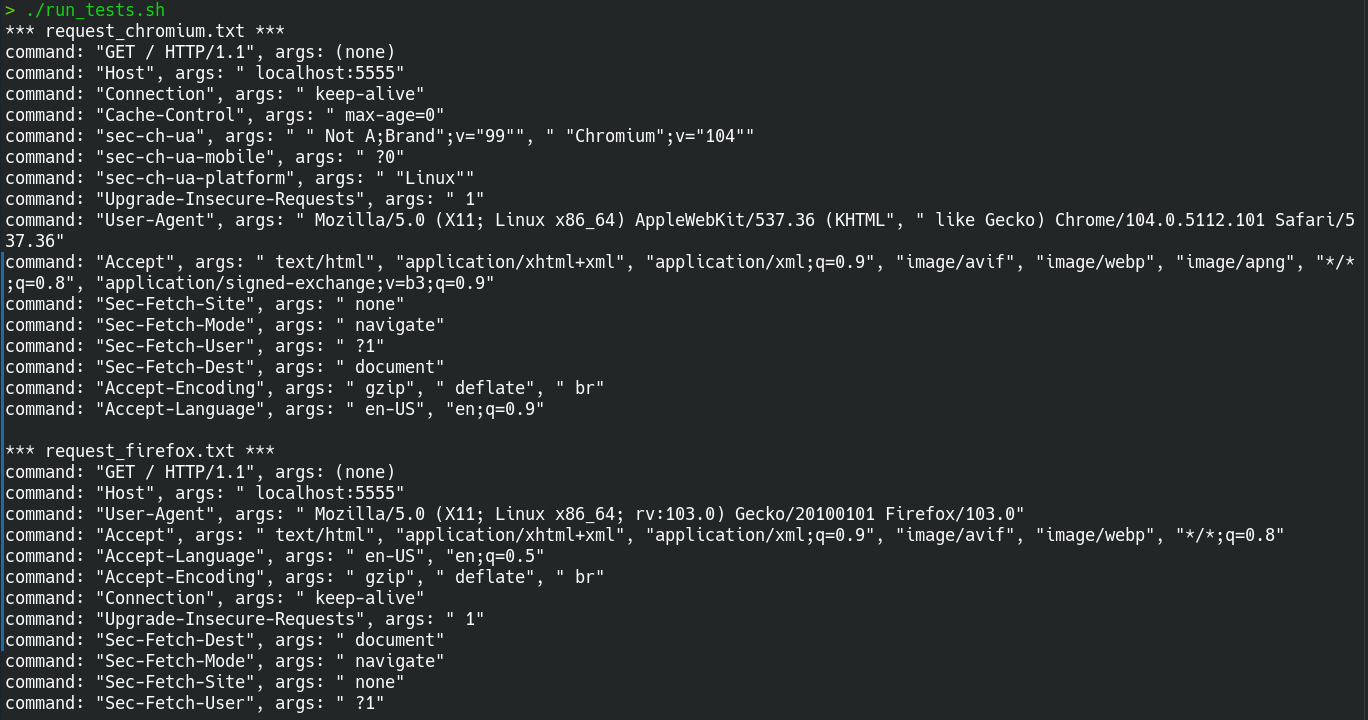
\includegraphics[width=\textwidth]{images/tests.png}
    \end{center}
\end{figure} 

\end{document}